\documentclass[conference,compsoc]{IEEEtran}

% *** CITATION PACKAGES ***
%
\ifCLASSOPTIONcompsoc
  % IEEE Computer Society needs nocompress option
  % requires cite.sty v4.0 or later (November 2003)
  \usepackage[nocompress]{cite}
\else
  % normal IEEE
  \usepackage{cite}
\fi
\ifCLASSINFOpdf
\else
\fi
\usepackage{amsmath}
\usepackage{algorithm,algpseudocode,float}
\usepackage{algorithmicx}
\renewcommand{\algorithmicrequire}{\textbf{Input:}}
\renewcommand{\algorithmicensure}{\textbf{Output:}}
\usepackage{array}
\usepackage{url}
\usepackage{lipsum}
\usepackage{graphicx}
\hyphenation{op-tical net-works semi-conduc-tor}
\usepackage{float} %要用这个宏包


\makeatletter
\newenvironment{breakablealgorithm}
{% \begin{breakablealgorithm}
	\begin{center}
		\refstepcounter{algorithm}% New algorithm
		\hrule height.8pt depth0pt \kern2pt% \@fs@pre for \@fs@ruled
		\renewcommand{\caption}[2][\relax]{% Make a new \caption
			{\raggedright\textbf{\ALG@name~\thealgorithm} ##2\par}%
			\ifx\relax##1\relax % #1 is \relax
			\addcontentsline{loa}{algorithm}{\protect\numberline{\thealgorithm}##2}%
			\else % #1 is not \relax
			\addcontentsline{loa}{algorithm}{\protect\numberline{\thealgorithm}##1}%
			\fi
			\kern2pt\hrule\kern2pt
		}
	}{% \end{breakablealgorithm}
		\kern2pt\hrule\relax% \@fs@post for \@fs@ruled
	\end{center}
}
\makeatother
\begin{document}
%
% paper title
% Titles are generally capitalized except for words such as a, an, and, as,
% at, but, by, for, in, nor, of, on, or, the, to and up, which are usually
% not capitalized unless they are the first or last word of the title.
% Linebreaks \\ can be used within to get better formatting as desired.
% Do not put math or special symbols in the title.
\title{Parallel distributed multi-objective fuzzy GBML}


% author names and affiliations
% use a multiple column layout for up to three different
% affiliations
\author{\IEEEauthorblockN{Keming Li, Liangyu Che}
\IEEEauthorblockA{School of Computer Science and Engineering\\
Southern University of Science and Technology\\
Email 11612126@mail.sustc.edu.cn\\
Email 11612228@mail.sustc.edu.cn
}}


% make the title area
\maketitle

% As a general rule, do not put math, special symbols or citations
% in the abstract
%\begin{abstract}

%\end{abstract}

% For peer review papers, you can put extra information on the cover
% page as needed:
% \ifCLASSOPTIONpeerreview
% \begin{center} \bfseries EDICS Category: 3-BBND \end{center}
% \fi
%
% For peerreview papers, this IEEEtran command inserts a page break and
% creates the second title. It will be ignored for other modes.
\IEEEpeerreviewmaketitle



\section{Introduction}
The basic purpose of this project is to base on [1] to implement a Parallel Distributed Multi-Objective Fuzzy Genetics-Based Machine Learning, which can be used to classify patterns.
\\
 \indent In this report, we introduce some primery of comparision results and conclusion.
\begin{itemize}
	\item Implement MOCCA(multi-objective cooperative coevolutionary algorithm).
	\item Implement random data dimension division method
	\item Implement a simple structure paralism GA structure, RING
	\item \textbf{Hybrid Fuzzy GBML}:We used python to build Hybrid Fuzzy GBML and run it successfully.
	\item \textbf{NSGA-II Framework}:We implemented the NSGA-II framework for individual sequencing.
	\item \textbf{PCA}:We implemented PCA to reduce dimension of data.
	\item \textbf{Parallel}:We implemented the island model to enable parallel computation.
	\item \textbf{Group cooperation}: Siyi Ding's group used our algorithm to train the fuzzy classifier as the classifier of his microwave recognition project.
	\item \textbf{Test}:We use Breast\_W, wine, sonar, pima, Glass and other data sets for training and testing. The results were close to [1].
\end{itemize}


\section{Background Knowledge }
\subsection{Evolutionary multi-objective optimization}

\subsubsection{Evolutionary algorithms}

\subsubsection{NSGA-II }

\subsection{Fuzzy rule-based classifiers}

\subsection{Coevolutionary algorithms}
Natural evolution is often thought of as a population living in a fixed environment, but this is not totally true. Due to the interaction between different species, changes in one species or group of species will affect other species to varying degrees. In biology, coevolution is used to indicate that species living in an environment try to survive depending one on each other.[3]\\
\indent Traditional evolutionary algorithms work on a fixed environments. In this case, the fitness of the individual is measured using a predefined fitness function. After several iterations, the evolutionary algorithm makes the individuals adapt to the environment according to the established fitness function.\\
\indent When the scale of the problem is too large, the traditional evolutionary algorithm will consume a large amount of hash power. At the same time, the whole system is inefficient and the results of each generation have low convergence.\\
\indent The basic idea of coevolutionary algorithms is divide and conquer, dividing a large problem into multiple interdependent subproblems called species. coevolutionary algorithms can be cooperative or competititive as well as interpopulation or intrapopulation. In coevolutionary algorithms, the evolving populations by cooperating with each other for the best fitness, individuals in the same species compete with each other to accelerate the convergence. \\
\indent coevolutionary algorithms has been also used to solve fuzzy rule classification problems.In the Michigan-style GBML framework, the rules are usually divided into distinct species according to the consequent. \\
\indent Multi-objective cooperative coevolutionary algorithm is one of cooperative coevolutionary algorithms (CCA).

\section{brief introduction of the original design}

\subsection{MOCCA}
There are five issues in MOCCA which are elaborated in this section: 
\begin{itemize}
	\item Problem Decomposition.
	\item Species Initialization
	\item Collaboration Formation.
	\item Fitness Evaluation.
	\item Framework.
\end{itemize}
\subsubsection{Problem Decomposition}
Since our project is based on Pittsburgh-style GBML framework, the problem could not be directly decomposed according to the consequence of rules.\\
\indent Our design method is similarly decompose the problem according to the consequence of rules. However, the individual is not a rule but a rule set in which the rules have the same consequence.
\begin{figure}[htbp]%current location
	\centering
	\scalebox{0.4}{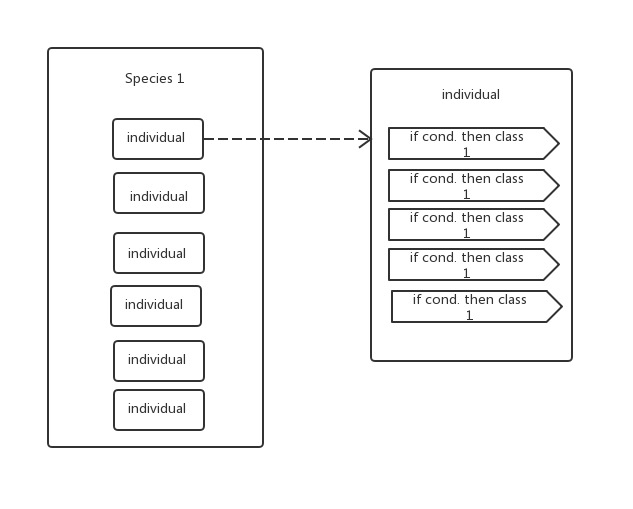
\includegraphics{species.png}}
	\caption{species \& individual}
	\label{species.png} 
\end{figure}
\subsubsection {Species Initialization}
we generate fuzzy rules with the training set, and the rules were then put into the their corresponding rule pools according to the consequence. Next, we randomly select M rules from one rule pool to generate an individual and put it into the corresponding species. 
\begin{figure}[htbp]%current location
	\centering
	\scalebox{0.3}{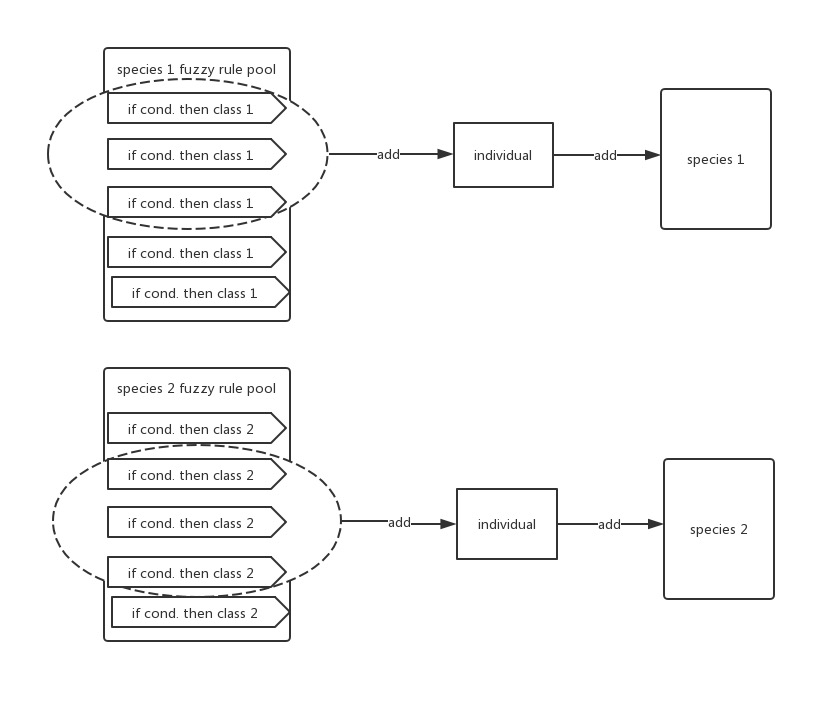
\includegraphics{init.png}}
	\caption{initialization}
	\label{initialization.png} 
\end{figure}
\subsubsection{Collaboration Formation}
The individuals in each species are not complete fuzzy classifier and cannot be evaluated directly. Therefore, in order to calculate the fitness of each individual, we need different species to cooperate. Forming collaboration requires the following two steps:
\begin{itemize}
	\item Representative selection 
	\item Combination operations
\end{itemize}
Before we evaluate individuals' fitness, we need to select the best individual and two random individuals from each species as representatives of the species. This operation is called representative selection.\\
\begin{figure}[htbp]%current location
	\centering
	\scalebox{0.6}{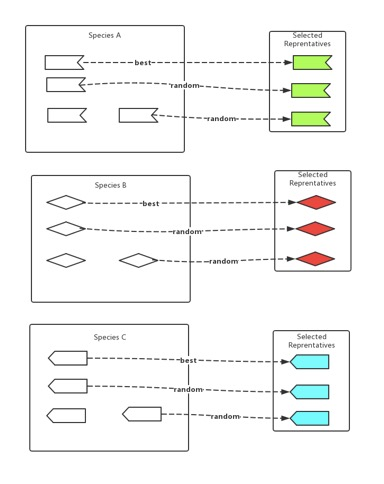
\includegraphics{selection.png}}
	\caption{Representative selection}
	\label{selection.png} 
\end{figure}
An individual will be merged with the optimal representative of other species to create a fuzzy classifier, and then two fuzzy classifiers will be created by merging the same method with the random representative of other species. This operation is called combination operations.\\
\begin{figure}[htbp]%current location
	\centering
	\scalebox{0.3}{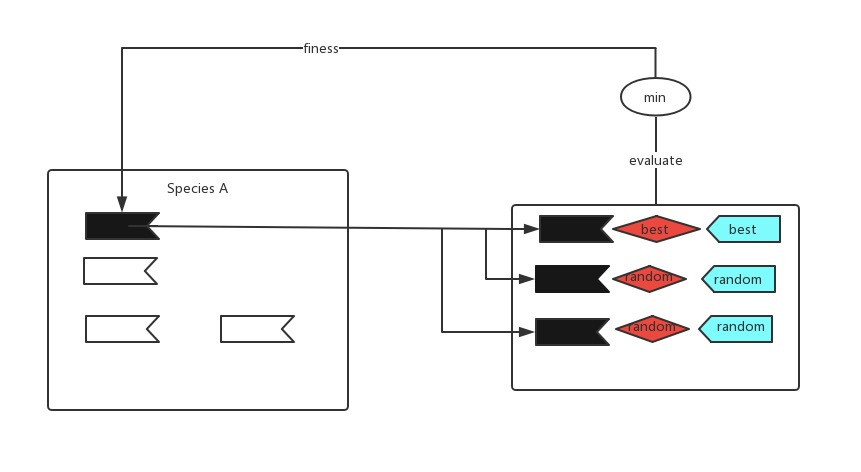
\includegraphics{combine.png}}
	\caption{Combination operation}
	\label{combine.png} 
\end{figure}
\subsubsection{Fitness Evaluation}
We calculate the fitness of the three fuzzy classifiers generated by Combination operations with the fitness function. Then, we select the lowest fitness as the fitness of the individual.

\subsubsection{Framework}
After initialized species, each species will evolve into offspring through Pittsburgh-style GBML. Then, we obtain the fitness of each individual through species collaboration. Next, enter the next evolution cycle until the end of evolution. Finally, we output the fuzzy classifier which composed of the best individuals in each species.
\begin{figure}[htbp]%current location
	\centering
	\scalebox{0.3}{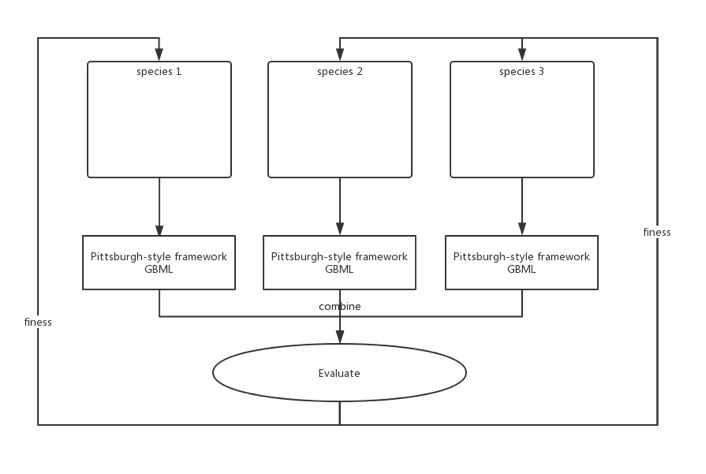
\includegraphics{framework.png}}
	\caption{Framework}
	\label{selection.png} 
\end{figure}
\subsubsection{Pseudocode}


\begin{breakablealgorithm}   
	\caption{MOCCA}  
	\label{alg:Framework} 
	\begin{algorithmic}[1]  
		\Require  
		$train\_data$
		\Ensure  
		$fuzzy\_classifier$ \\
		\State Species\_list $\gets$ Initial(train\_data)
		\While {gen $<$  N\_gen }
		\For {Species $\in$  Species\_list}
			\State SortWithFitness(Species)
			\State Species $\gets$ Species[:N]
		         \State representative\_list $\gets$ representative\_select(Speices)
			\While {offspring.length $<$  N }
				\State parent $\gets$ Binary\_select(Species)
				\State child $\gets$ Crossover(parent)
				\State mutate(childs)
				\State offspring $\gets$ child
			\EndWhile
			\State Species $\gets$ offspring
		\EndFor
		\For {Species $\in$  Species\_list}
			\For {individual $\in$ Species\_list}
				\State classifier $\gets$ Combine(individual, representative\_list)
				\State individual.Fitness $\gets$ fitness\_func(classifier,train\_data)
			\EndFor
		\EndFor
		\EndWhile
		\State fuzzy\_classifier $\gets$ best\_combine(Species\_list)
		\State \Return{$fuzzy\_classifier$}
	\end{algorithmic} 
\end{breakablealgorithm}


\section{Experimental results}
\subsection{Decomposition Strategy}
The following data were measured on a supercomputer.\\
\indent Select wine\_change and Glass as data sets\\
\indent Label decomposition: each subpopulation size is 30, run 150 generations.\\
\indent Dimensional decomposition:  each subpopulation size is 100, run 150 generations.\\

\indent The tables below compare the performance of the two algorithms in wine\_change and glass
\begin{table}[H]
	\centering
\begin{tabular}{ccc}
\hline
algorithm& avg generation time& total time\\
\hline
Label decomposition& 12.32s& 1903.5s\\
Dimension decomposition& 0.87s& 139.2s\\
\hline
\\
\end{tabular}
\caption{performance in wine change}
\end{table}


\begin{table}[H]
	\centering
\begin{tabular}{ccc}
\hline
algorithm& avg generation time& total time\\
\hline
Label decomposition& 4.67s& 724.6s\\
Dimension decomposition& 1.49s& 236.8s\\
\hline
\\
\end{tabular}
\caption{performance in Glass}
\end{table}
The following figures show the time spent per generation in the wine\_change and glass and the process communication time.
\\\\\

\begin{figure}[htbp]%current location
	\centering
	\scalebox{0.3}{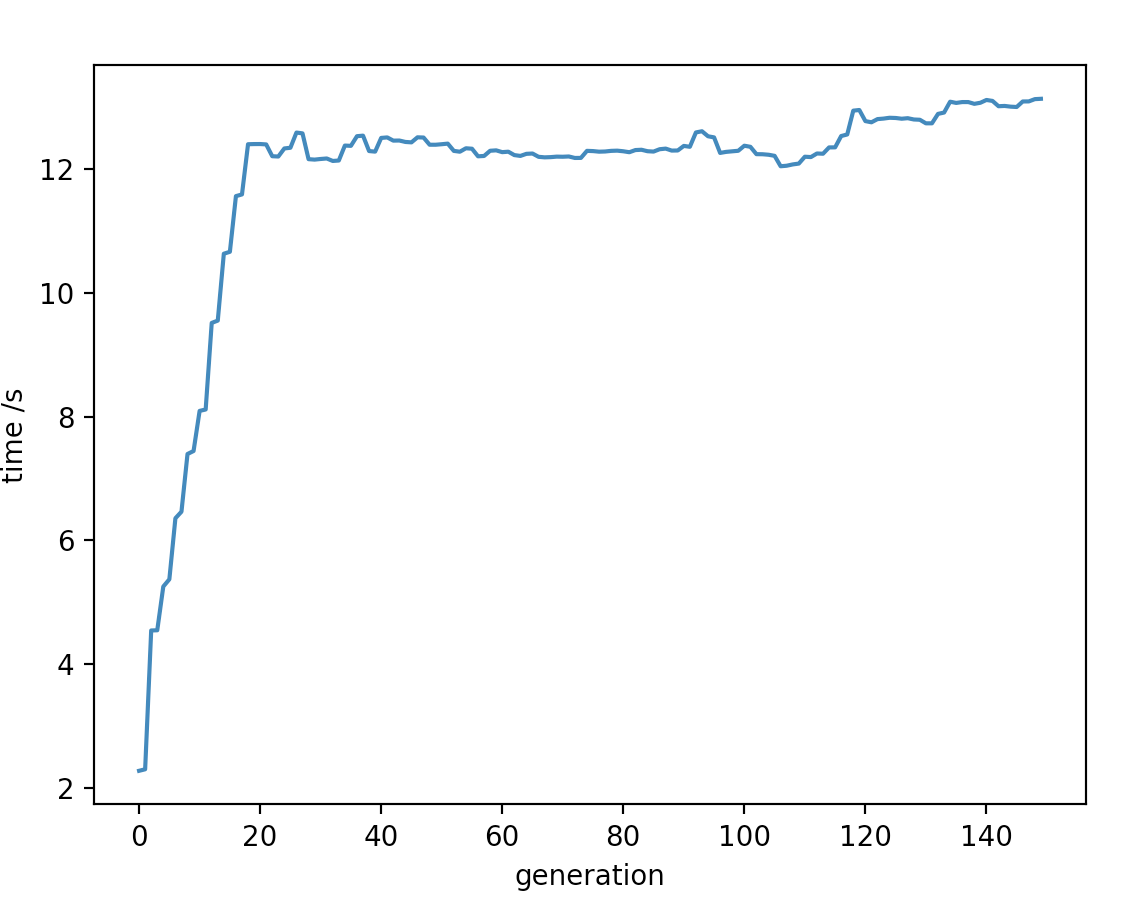
\includegraphics{w_label_gen.png}}
	\caption{label\_decomposition\_wine\_generation\_time}
\end{figure}

\begin{figure}[htbp]%current location
	\centering
	\scalebox{0.2}{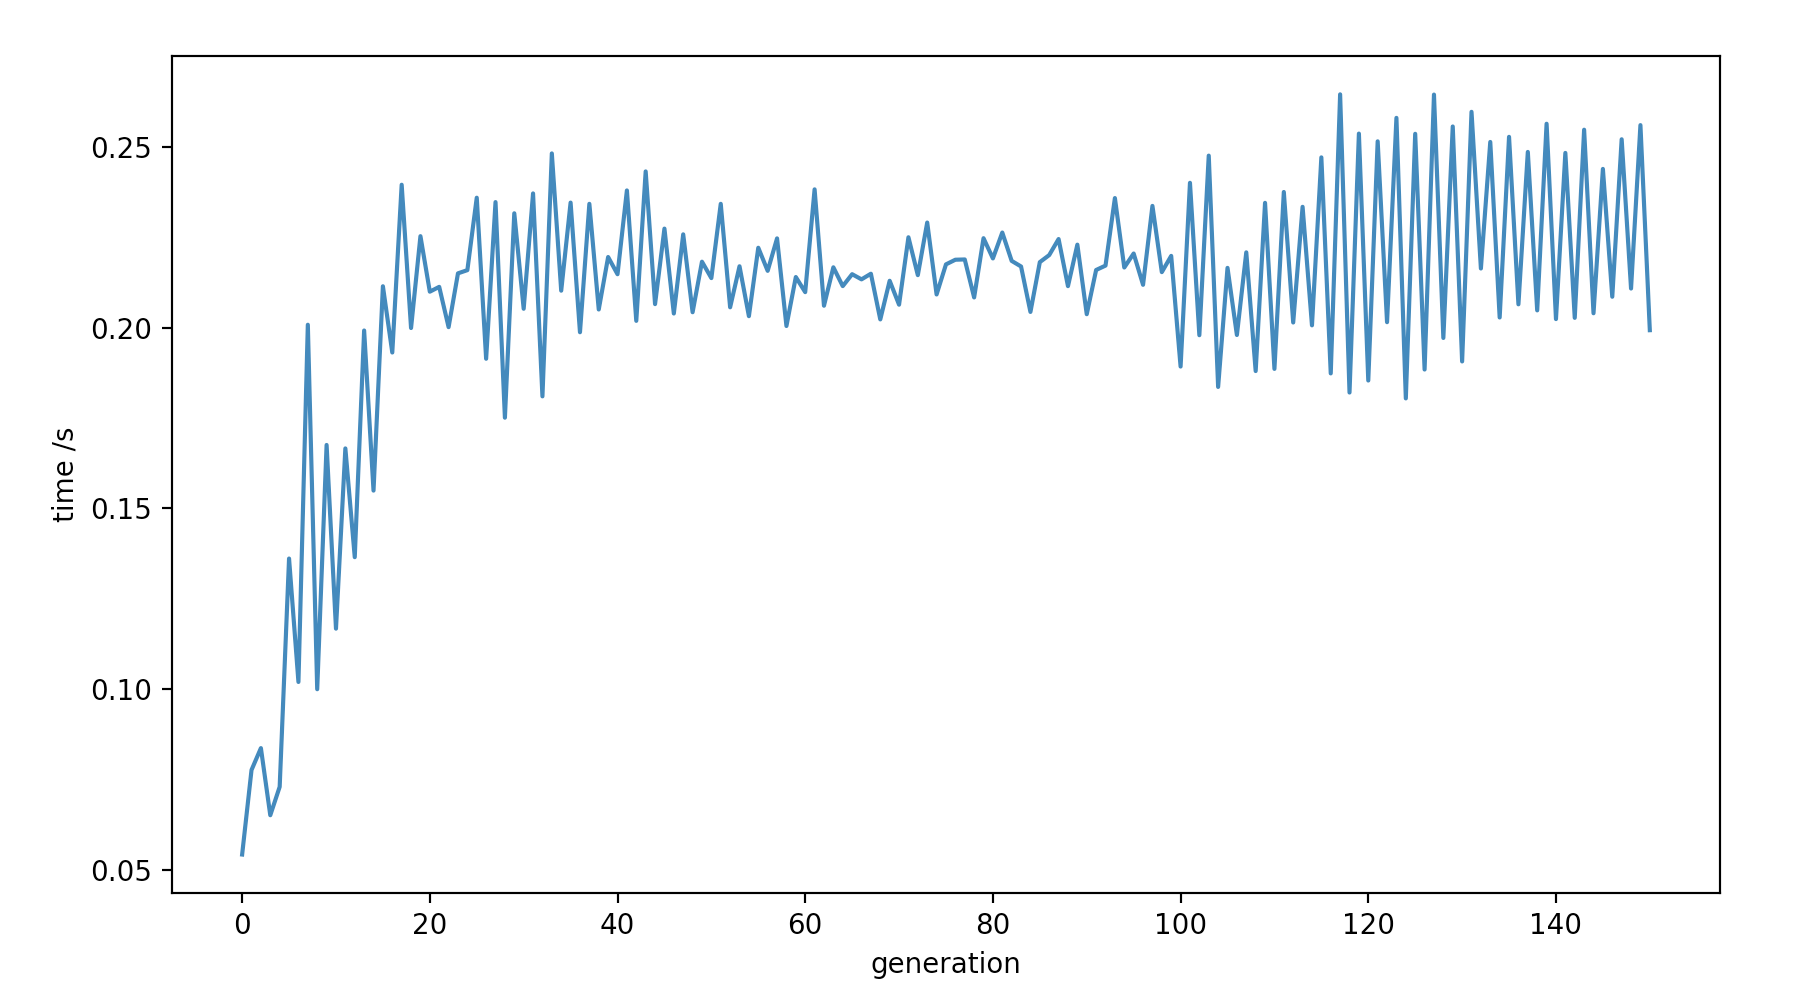
\includegraphics{w_label_com.png}}
	\caption{label\_decomposition\_wine\_communication\_time}
\end{figure}

\begin{figure}[htbp]%current location
	\centering
	\scalebox{0.3}{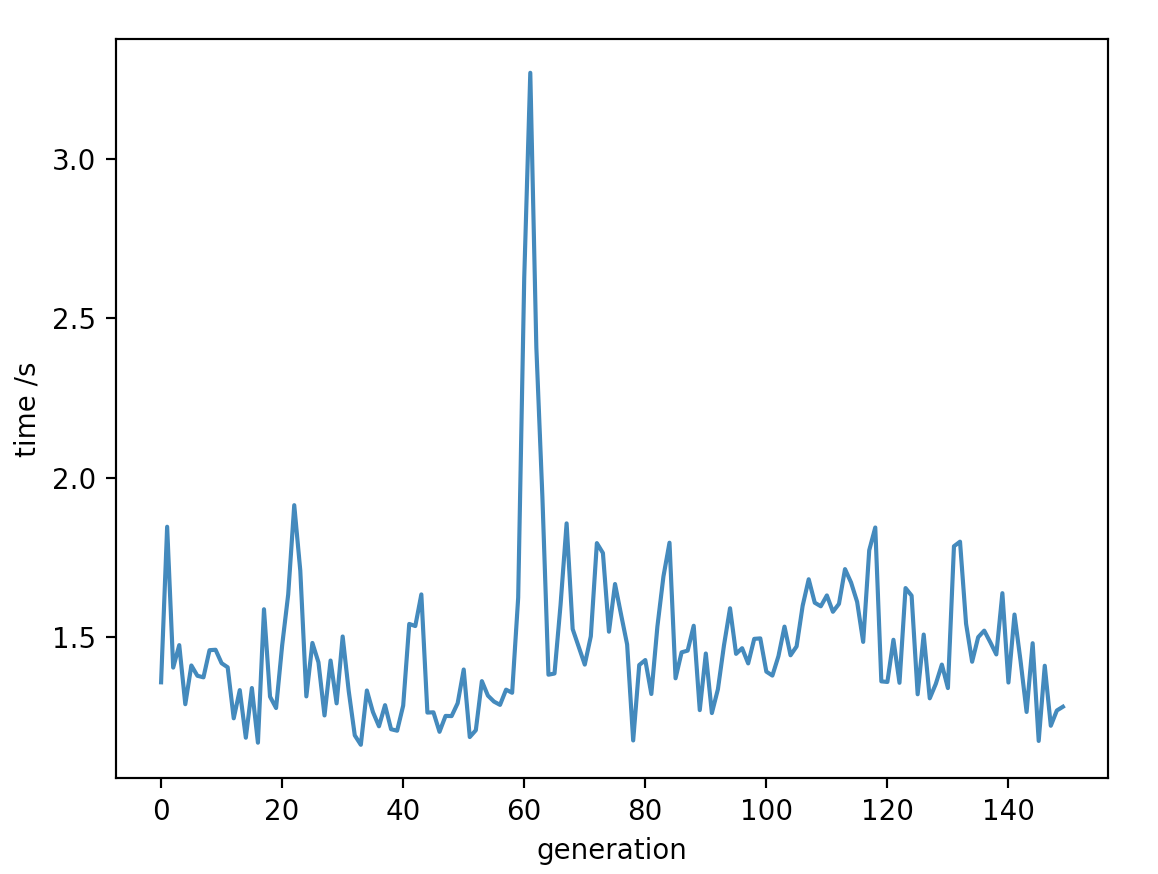
\includegraphics{w_dim_gen.png}}
	\caption{dim\_decomposition\_wine\_generation\_time}
\end{figure}

\begin{figure}[htbp]%current location
	\centering
	\scalebox{0.3}{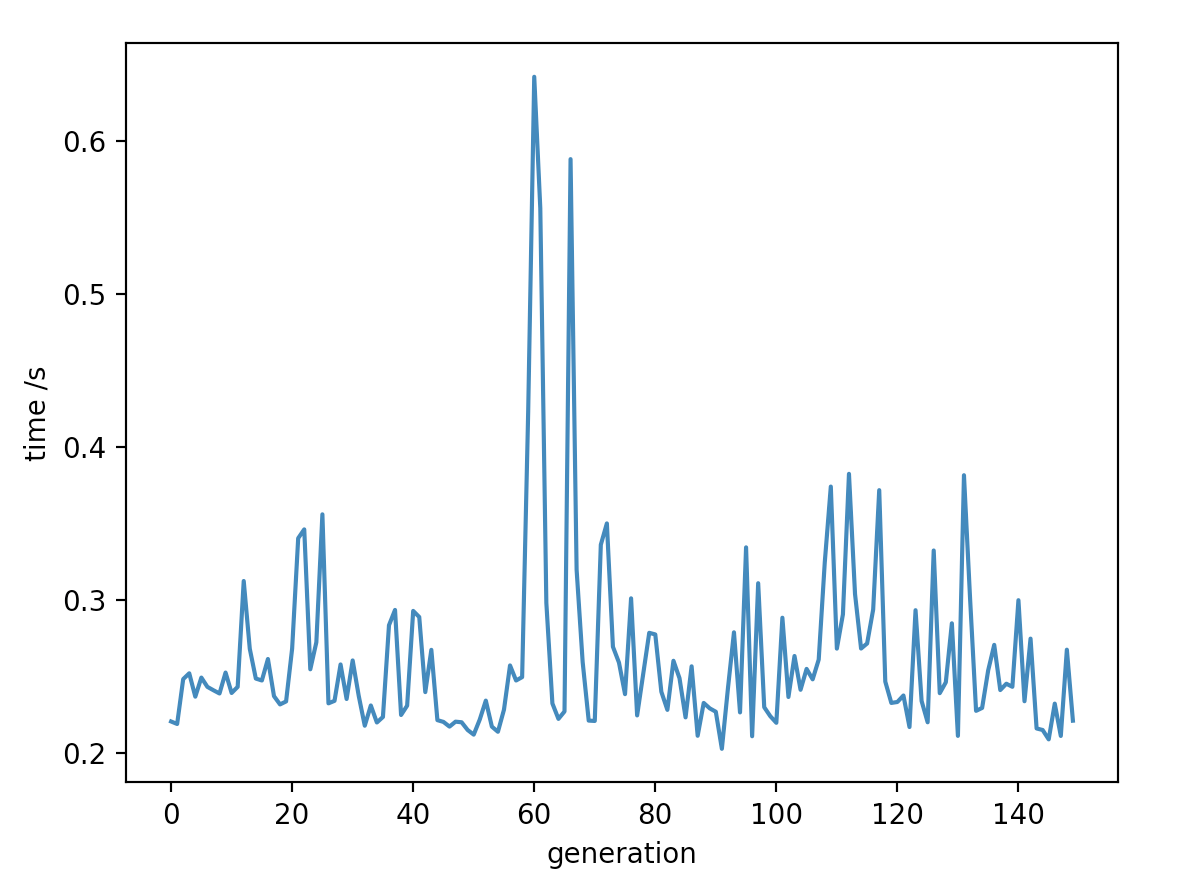
\includegraphics{w_dim_com.png}}
	\caption{dim\_decomposition\_wine\_communication\_time}
\end{figure}

\begin{figure}[htbp]%current location
	\centering
	\scalebox{0.3}{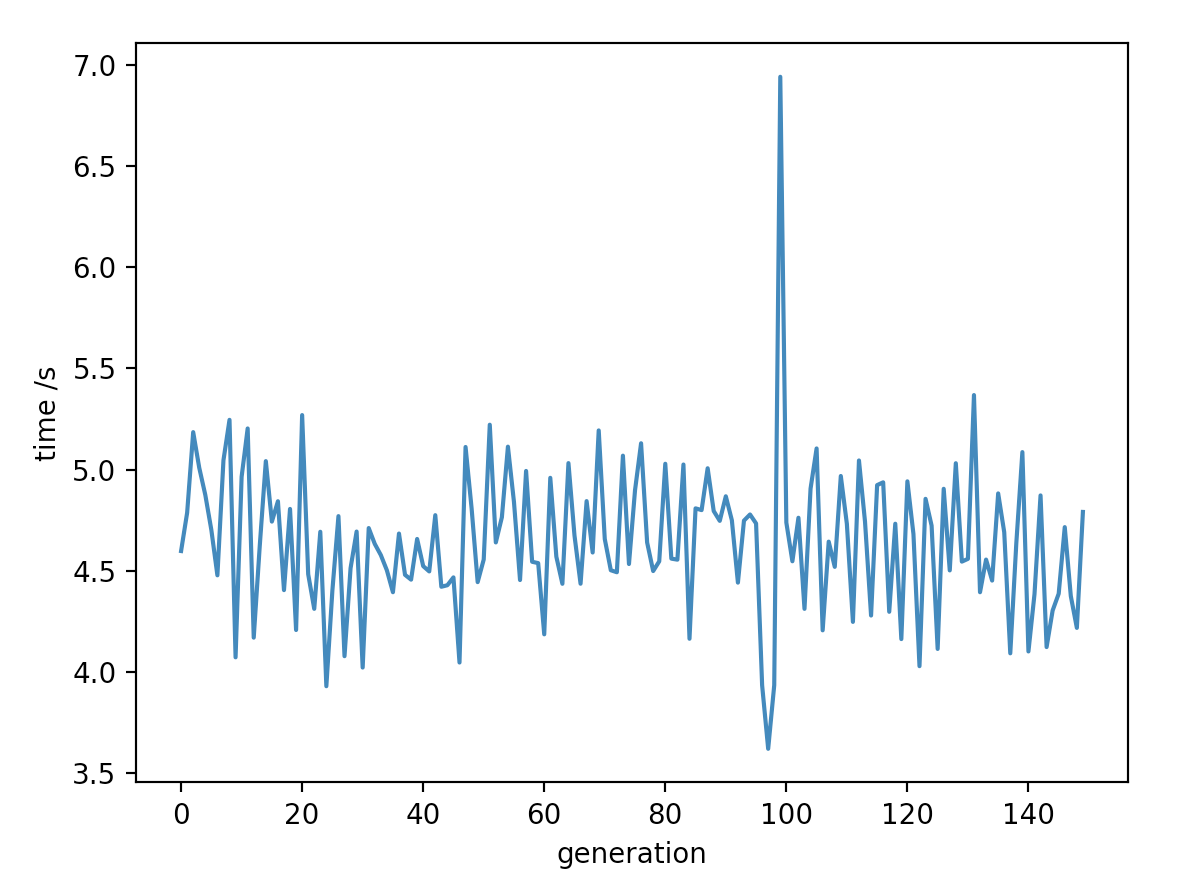
\includegraphics{g_label_gen.png}}
	\caption{label\_decomposition\_glass\_generation\_time}
\end{figure}

\begin{figure}[htbp]%current location
	\centering
	\scalebox{0.3}{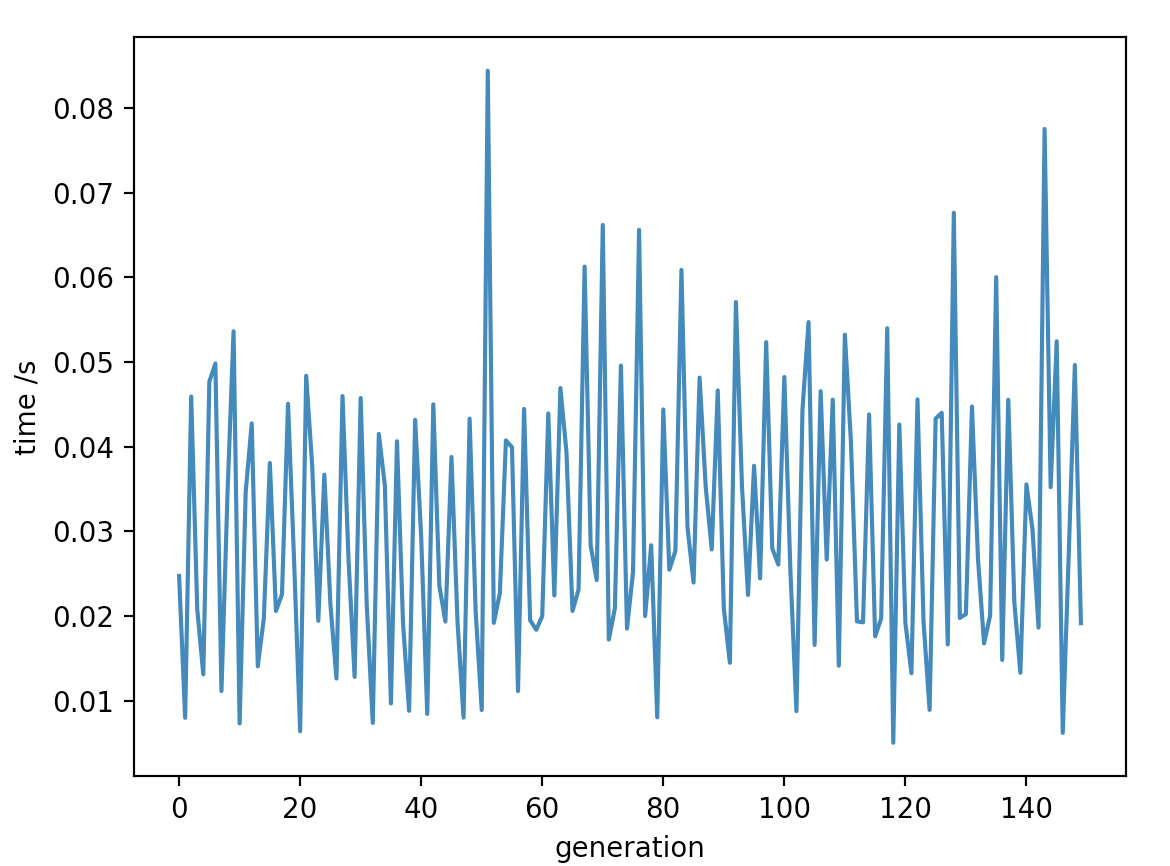
\includegraphics{g_label_com.png}}
	\caption{label\_decomposition\_glass\_communication\_time}
\end{figure}

\begin{figure}[htbp]%current location
	\centering
	\scalebox{0.3}{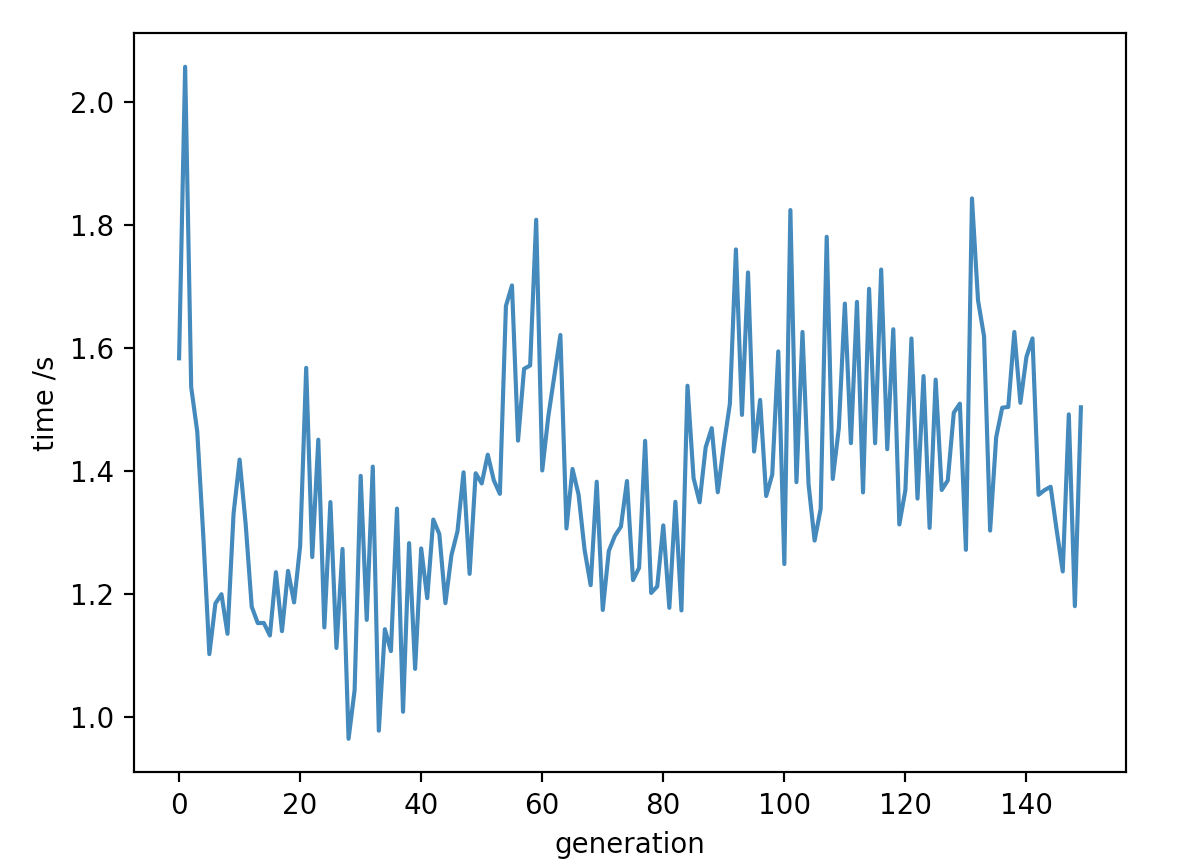
\includegraphics{g_dim_gen.png}}
	\caption{dim\_decomposition\_glass\_generation\_time}
\end{figure}

\begin{figure}[htbp]%current location
	\centering
	\scalebox{0.3}{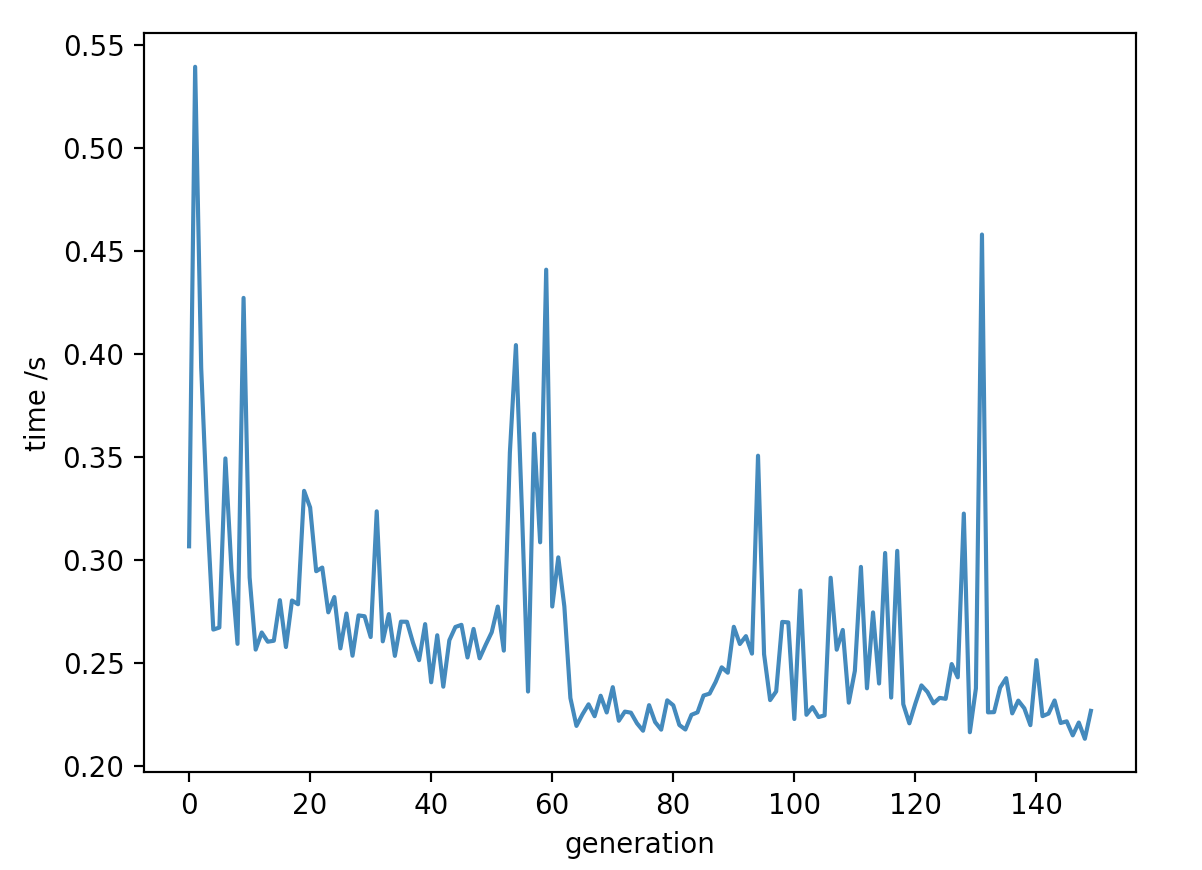
\includegraphics{g_dim_com.png}}
	\caption{dim\_decomposition\_glass\_communication\_time}
\end{figure}
\section{Analysis of experimental results and hypothesis}
\subsection{Decomposition Strategy}
\subsubsection{Comparison of run time of different algorithms}
\indent When using label decomposition, the individual of a single subpopulation is not a complete classifier, and the classifier generated by combining the subpopulation needs to be reevaluated in each generation, which takes a lot of time. \\
\indent However, for dimension decomposition, the individual of each subpopulation is the classifier that only classify the specific dimensions (the other dimensions are don't care). In this way, when cooperating, it only needs to recombine the subpopulations within the main process in ten generation, which consumes less time.
\subsubsection{Comparison of run time in different datasets}
\indent For label decompositon, the algorithm run faster in the multi-label dataset  than in the small-label dataset when those datasets size and dimension are equal.


\begin{thebibliography}{1}
\bibitem{reference} 
H. Ishibuchi and Y. Nojima, “Analysis of interpretability-accuracy tradeoff of fuzzy systems by multiobjective fuzzy genetics-based machine learning,” International Journal of Approximate Reasoning, vol. 44, no. 1, pp. 4-31, January 2007.
\bibitem{reference} 
X. Yao, Evolving Artificial Neural Networks in Proceedings of the IEEE, vol. 87, no. 9, pp. 1423–1447,September 1999
\bibitem{reference} 
Xing Zong-Yi, Hou Yuan-Long, Zhang Yong, Jia Li-Min and Hou Yuexian, "A Multi-objective Cooperative Coevolutionary Algorithm for Constructing Accurate and Interpretable Fuzzy systems," 2006 IEEE International Conference on Fuzzy Systems, Vancouver, BC, 2006, pp. 1404-1410.


\end{thebibliography}


% trigger a \newpage just before the given reference
% number - used to balance the columns on the last page
% adjust value as needed - may need to be readjusted if
% the document is modified later
%\IEEEtriggeratref{8}
% The "triggered" command can be changed if desired:
%\IEEEtriggercmd{\enlargethispage{-5in}}

% references section

% can use a bibliography generated by BibTeX as a .bbl file
% BibTeX documentation can be easily obtained at:
% http://mirror.ctan.org/biblio/bibtex/contrib/doc/
% The IEEEtran BibTeX style support page is at:
% http://www.michaelshell.org/tex/ieeetran/bibtex/


%\end{thebibliography}





% that's all folks
\end{document}


